% -*- mode: Latex -*-
% Time-stamp: "2015-02-18 17:55:40 sb"

\documentclass[twocolumn,aps,pra,showpacs,preprintnumbers,bibnotes]{revtex4-1}

\usepackage[T1]{fontenc}

\usepackage{natbib}
\usepackage{graphicx}
\usepackage{bm}
\usepackage{color}
\usepackage{amsmath}

%% Keep track of changes
%\usepackage[final]{changes}
\usepackage[draft]{changes}
\definechangesauthor[color=green]{AM}
\definechangesauthor[color=blue]{SB}

\DeclareMathOperator{\re}{Re}
\DeclareMathOperator{\im}{Im}

\newcommand\avg[1]{\left\langle#1\right\rangle}

\newcommand\unit[2]{\ensuremath{#1~\mathrm{{#2}}}}

\newcommand\Ket[1]{\ensuremath{|{#1}\rangle}}
\newcommand\Bra[1]{\ensuremath{\langle{#1}|}}

\newcommand\Isotope[2]{\ensuremath{^{#1}\mathrm{#2}}}
\newcommand\Li{\Isotope{6}{Li}}
\newcommand\K{\Isotope{40}{K}}
\newcommand\Rb{\Isotope{87}{Rb}}
\newcommand\Sr{\Isotope{87}{Sr}}
\newcommand\Yb{\Isotope{171}{Yb}}
\newcommand\Er{\Isotope{167}{Er}}
\newcommand\Dy{\Isotope{161}{Dy}}

\renewcommand{\vec}[1]{\ensuremath{\bm{#1}}}

\newcommand\NA{\ensuremath{\mathrm{NA}}}
\newcommand{\osim}{\ensuremath{\mathord{\sim}}}
\newcommand{\Erecl}{\ensuremath{E_\mathrm{rec}}}
\newcommand{\Ereca}{\ensuremath{E_\mathrm{rec}^\mathrm{(a)}}}
\newcommand\FIXME{{\color{red}\ensuremath{\mathrm{FIXME}}}}

\newcommand\TrapFreq{\ensuremath{\nu_t}}
\newcommand\RecoilEnergy{\ensuremath{E_\mathrm{rec}}}

\graphicspath{{./figures/}}
\begin{document}

\title{Design and Implementation of Stable High Power Optical Lattices for Quantum Gas Microscopy}


\author{Li Microscope Collective}
\author{M. Greiner}
\affiliation{
  Department of Physics, Harvard University,
  Cambridge, Massachusetts, 02138, USA}

\date{\today}
\begin{abstract}
We describe the design of a stable high power 1064 nm laser for use in optical lattice experiments. The system is based on a high quality mephisto NPRO seeding an array of four heavily modified fiber amplifiers. The intensity of every beam is stabilized with a low noise, nonlinear feedback system, and the waist can be smoothly controlled. 
\end{abstract}
\maketitle
\section{Introduction}
Ultracold atoms in optical lattices have become a powerful platform for experiments ranging from investigations of strongly correlated systems, quantum state engineering, quantum computing architectures and precision metrology, among others.
Further, the recent advent of quantum gas microscopy has enabled studies that exhibit unprecedented control over few atom systems that function at extremely low energy scales.
However, this rapid progress places ever more stringent technical constraints on the lasers used to trap and manipulate the atomic systems.
For example, in experiments at low temperatures, heating due to the intensity noise of a lattice cannot be allowed to approach the thermalization timescales lest the system fail to thermalize at the required temperature.
Similarly, experiments that rely on a small number of atoms held by multiple traps places stringent requirements on the relative stability of the traps.
We demonstrate a high power lattice system that exhibits levels of intensity noise below -120 dBc between 1 kHz and 3 MHz, and is positionally stable at the XXX site level. 
This system has been successfully used in a Fermi gas microscope to investigate the charge and spin sectors of the Hubbard model with unprecedented control. 
\begin{figure}
    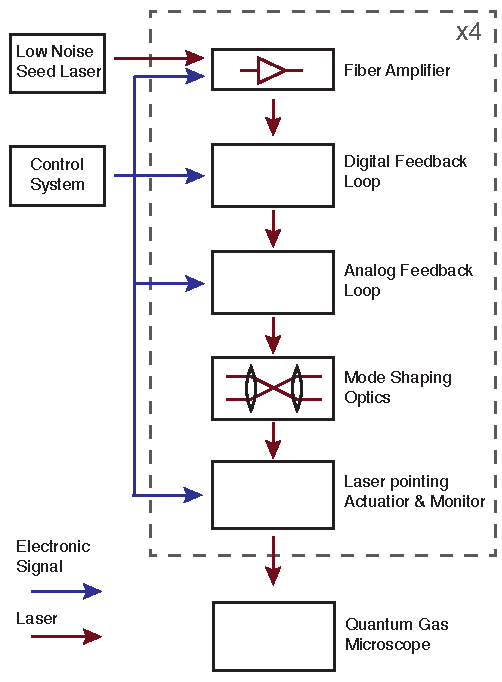
\includegraphics{figures/figure1/figure1.pdf}
    \caption{High level overview showing the major components of the lattice laser feedback system}
\end{figure}


\section{High level Overview}
The system requirements:

The architecture of the system is based on a single low-power, low-noise seed laser that supplies light to an array of four high-power fiber amplifiers.
These amplifiers provide a sufficient amount of light but also substantially increase the noise of the light and degrade the mode shape. 
The fiber amplifier output provides light is controlled to two feedback 

\section{Mephisto}
The lattice laser system is seeded by an Innolight Mephisto laser, which provides approximately 2 W of 1064 nm light. 
This commercial laser utilizes a non-planar ring oscillator (NPRO) design that ensures superb phase and intensity stability. This source is split into four fibers (Thorlabs XXX) by means of polarizing beam splitters, where two of the fibers are detuned from each other by XXX MHz, to prevent interference of the lattice beams. Figure 1 shows the mechanical layout of this system, as well as the intensity noise performance (see supplementary material).


\section{Nufern Fiber Amplifiers}
Quantum gas microscopy of Li requires single site trap frequencies of approximately 1 MHz \cite{Parsons2015}.
Such trap frequencies may only be attained using tightly focused high power beams, which requires that the seed power be amplified to approximately 30 W per lattice axis, which is done using Nufern Fiber amplifiers (PART NUMBER XXX).
These amplifiers can amplify 150 mW to up to approximately 45 W (depending on pump diode current) by using a length of fiber doped with XXX (erbium or ytterbium) and pumped with xxx nm light from fiber coupled diode sources to provide a gain medium for 1064 nm light. 
The amplification is performed using a two stage amplifier design, where the stages are contolled using separate power supplies and electronics.
The high powers supplied by the fiber amplifiers raise two engineering difficulties. First, the fiber amplification process is inherently noisy, due to acoustic coupling of the fiber to the environment, electrical design of the amplifier, and spontaneous Brillouin scattering (SBS). 

The NUFERN MODEL NUMBER suffers from several problems: it is controlled via a USB interface, requiring a digital ground on the control PCB inside the device. Further, this digital ground is not isolated from the remainder of the electronics leading to potential ground loops between the controlling computer and the fiber amplifier. 
We solve this problem by replacing the USB control board with a custom-designed, ethernet based solution that is compatible with our custom control system. 
There are two power supplies in the fiber amplifier - a general purpose supply for the control electronics and first stage and a high current supply for the second stage. 
Further, despite the presence of a water-cooled coldplate to cool the fiber and pump diodes, the high power supply is air cooled using a fan approximately 20 cm away from the gain fiber and has been thought to lead to increased noise at acoustic frequencies.
To reduce acoustic coupling and reduce switching power supply noise, both power supplies were removed from the fiber amplifier enclosure, the low power supply was replaced by acopian XXXX PSU and the high power supply was filtered using an XXX line filter.
Combined, these changes serve to suppress certain noise spurs measured in the relative intensity noise (RIN) of the fiber amplifier, as seen in figure 1. 
The measurements were carried out on a single fiber amplifier, prior to and after the modifications. The initial and final noise spectra were verified to be consistent between amplifiers coming from the same manufacturing batch.

(WARNING: THIS SECTION IS BEING BUILT) The operation of the Nufern fiber amplifiers can be further optimized by finely controlling the cooling water required, by tuning the waveleng of the light supplied by the diodes that optically pump the gain fiber.
Optimizing the temperature is advantageous because (1) the maximum output power of the fiber amplifier is increased due to the improved efficiency of the pump light and (2) the lifetime of the device is increased because less stray pump light needs to be absorbed when the pump light is separated from the desired light, reducing the thermal load. 
This is possible because the pump diodes are fixed directly to the water-cooling plate without temperature regulation.
Adding a Peltier TEC and regulating to the optimal wavelength is possible, but is technically difficult as it requires large cooling power of $\approx100$ W per each of the three pump diodes and the associated complexity of three feedback loops.
We use a single XXX heat exchanger to supply cooling water to an array of four fiber amplifiers and tune the temperature such that the average power supplied by the amplifiers supplying the $X$ and $Y$ lattices is optimized.


\section{Mode and beam shaping}
The free-space propagation of the fiber amplifier output presents several challenges (1) the high power is sufficient to induce substantial thermal lensing, (2) the positional fluctuations of the waist at the atoms cannot exceed 
a few microns from shot to shot, (3) by construction, the beam is retroreflected, which threatens the lifetime of the amplifier unless sufficient isolation is used (4) approximately 1 W of power leaks into the undesired cladding modes of the fiber. 
To condition the beam into a desired shape, a train of optical elements is used, shown in figure \ref{fig:opticalelements}, which shapes the beam. 
Due to the high laser power, fused silica glass is used everywhere but in the acousto-optic modulator, Berek compensator and optical isolators, to minimze thermal lensing.
For the same reason, IBS coatings are used wherever possible, due to the higher damage thresholds.
Further, even small reflections pose both a danger to the users and the thermal equillibrium of the system.
To alleviate this danger, all undesired beams above a 100 mW are directed to water cooled beam-dumps that are removed from the beam paths as far as possible.

The large-diameter fiber tip is mounted in a monolithic, oxygen-depleted copper mount, and the beam is collimated using an XXX 20 mm fused-sileca triplet collimator from Opto-Sigma, which produces a beam with $m^2 = XXX(X)$.
Then, the polarization is cleaned up using an IBS coated Brewster plate polarizer, which has the added benefit of rejecting the undesired cladding modes. 
The fact that the lattice is retro-reflected, combined with the observation that optical isolation falls with applied optical power\cite{LIGO} means that two stages of optical isolators must be used. The optical isolators are based on the 5 mm diameter Faraday rotators from Thorlabs. 
The optical isolators are located approximately 1 m away from the ultracold atomic system, meaning that undesired stray fields can have a dramatic effect.
To overcome this problem the isolators are enclosed in mu-metal shielding, reducing the field outside the can by an estimated factor of XXX.

\section{High power feedback}

After the beam has been cleaned up and isolated, it is important to consider two aspects of the desired experiment: (1) the lattice power must be continuously tunable from around 10 $\mu$W to around 20 W, (2) the location of the minimum gaussian beam waist must be accurately positioned to overlap the other lattices and dipole traps present in the experiment, and must remain there for the duration of the collection process (typically hours).
To appease the first of these requirements, a two-stage feedback system is implemented. The reason for the two stages is simple: the experiment typically operates in one of two regimes, which we will term \textit{detection} and \textit{interaction}. 
In the interaction phase of the experiment, the lattice is relatively shallow (depths of $\approx 10 E_R$, where $E_R$ is the geometric recoil of the lattice), allowing atoms to tunnel and interact with other atoms. 
In this regime, fine and potentially fast control is required.
In the detection phase, the depth of the lattice is dramatically raised ($\approx 2000 E_R$), isolating atoms in their individual wells so that Raman sideband imaging can be performed \cite{parsons2015}.
In this regime, the control need not be fast, and the passive stability of the Mephisto laser ensures that noise is low at relevant frequency scales.
Thus, two loops are utilized, a fast loop that uses an acousto-optic modulator to actuate the laser power at low powers, and a slow loop which uses a Berek compensator, to actuate in the high power mode.

After the isolation stage, we use the sequence of optical elements shown in figure \ref{fig1}, consisting of a polarizer, half-wave plate (HWP), Berek compensator mounted on a precision galvo (Thorlabs XXX) half-wave plate, and polarizer. The berek compensator is a simple $z$-cut quartz plate coated to be anti-reflecting at 1064 nm. 
By tilting the plate about its vertical axis, the extraordinary axis is mixed into the propagation of the beam, leading to a tilt-dependent bi-refringence that can be tuned from a zero-wave plate past a half-wave plate.
Combined with the surrounding polarization optics, rotation of the Berek compensator changes the transmitted power with perfect contrast and transmitted power as a function of the tilt angle is shown in figure \ref{fig2}.
If the half-wave plates in the Berek compensator are tuned to precisely 45 degrees from the angle of the tilt, the modulation contrast of the transmission is perfect, however, we purposefully detune from this configuration such that the minimum power transmitted through this system is approximately 1 W for each lattice axis. 
Thus, when the system is in \textit{interaction} mode, tilt noise on the Berek compensator is strongly suppressed by positioning the system at the minimum.
Naturally, rotation of a parallel plate in the beam path induces a shift of the beam, but this is acceptable because the Berek compensator is only active during the imaging phase of the experiment, when the position of the underlying harmonic trap is largely irrelevant.

Past the Berek compensator we high power TeO$_2$ AOM (part number XXXX), where the power of the RF supplied to the AOM is used to actuate the fast, low power feedback loop.
The AOM material is chosen for its ultra-low thermal lensing and easily-accessible required RF powers, and the AOM itself is mounted on a custom-built, monolithic, water-cooled flexure mount that allows optimization of the AOM efficiency, but that has been found to be stable over approximately two years of operation.
The local oscillator (LO) RF source is a custom-built printed circuit board (PCB) using a phase locked loop (PLL) based on the ADF4002 IC and XXX voltage controlled oscillator (VCO), preamplified with the XXX low noise amplifier. 
This RF power is actuated using a mixer (Minicircuits XXX), which functions down to DC and a high-isolation RF switch (Minicircuits XXX), followed by a power amplifier stage (RF-bay XXX). After the AOM, the beam is sampled twice using a single beam sampler (Thorlabs BSF-10C), by taking the reflections from the front and rear facets of the optic, which are conveniently angled away from each other by XXX.
One of the sampled beams is further attenuated by a factor of approximately 4\% by reflecing off an uncoated fused-silica plate, and the two sampled beams are directed toward a pair of identical photo-diodes. 


\section{Photodiodes}
Fast, low-noise photodiodes are required both to provide the monitoring arm of the feedback loop and to characterize the RIN of the system.
An ideal device would have a bandwidth up to approximately 3 MHz, with a noise floor below approximately -150 dBc over that range.
To approach these specifications, we use a custom designed PCB that implements a simple trans-impedance amplifier in a convenient physical package, providing a bandwidth (BW) between XXX and XXX, depending on the transimpedance gain, which can be set by a resistor. 
The photodiode can be safely operated up to incident powers of approximately 10 mW, which sets a XXX dBc shot noise limit on the RIN that can be detected.
A photodiode with a BW of XXX MHz is used to characterize the system, while photodiodes with a bandwidth of XXX and correspondingly higher gain are used for feedback.

The chosen photodiode (Hamamatsu XXX) is an InGaS based, small-area, low-noise design with a high efficiency at 1064 nm.
Prior to use, the protective window is removed from the photodiode to prevent interference effects.
Further, to reduce the capacitance of the system, a reverse bias of XXX V is applied to the photodiode by a temperature-stabilized voltage reference (Digi-key XXX).
The transimpedance circuit is shown in figure XXX - it converts the photo-current supplied by the photodiode to a voltage signal using the low noise XXX operational amplifier. 
The electronic assembly is housed in a metal enclosure to minimize interference effects, but is mounted to the optical table using isolating mica posts, to prevent ground loops. 

Light is focused onto the photodiode using a 25.4 mm lens such that the beam at the photodiode is significantly smaller than the photodiode diameter, to prevent pointing fluctuations from registering as positional fluctuations. 
An iris and interference filter (Semrock XXX) are used to elimnate stray sources of light. 

\section{Loop Filter}
Having covered the actuation and monitoring mechanisms of the feedback system, the only remaining part is the loop filter component of the feedback circuit, which compares the \textit{setpoint} signal supplied by the experimental control system, $v_s(t)$ and the monitoring signals $v_m(t)$, to adjust the actuation accordingly.
We use a simple, purely integrating design based on the XXX opamp, in three stages, as seen in figure XXX.
The first stage computes an error signal, $e(t)=v_m(t)-v_s(t)$, which is integrated by the second stage, with a manually tunable gain, set by a low-drift trimpot (digikey xxx). 
The third stage is used to accomodate the fact that the actuation arm is in nonlinear - the optical power transmitted by the AOM is proportional to the RF power incident on it $P_{\mathrm{rf}}\propto v_{if}^2$, where $v_{if}$ is the actuation signal supplied to the IF port of the mixer.
In effect, if the rest of the feedback system was linear, this would correspond to a quadratically increasing gain until the AOM is saturated, which could lead to slow behavior at low signal levels and ringing at higher signal levels.
Thus, the third amplification stage primarily serves to approximately linearize the response of the feedback system by increasing the gain at low signal levels and suppress it at high signal levels, which is accomplished by adding a diode (Digi-Key XXX) in series with a resistor $R_h$ in parallel to the usual gain resistor $R_l$ in the feedback arm of the operational amplifier. 
This can be clearly seen to acheive the desired effect in two exreme cases - far below the diode drop, the diode is an open circuit and the gain is set by $R_l$, where above the diode drop it is a closed circuit where the gain is set by the resistor $R_h$.
Naturally, the voltage drop over the diode is chosen such that it is approximately half the maximum desired signal level of the photodiode (3.3 V).
Another function of the last stage is to clamp the voltage to zero, in order to prevent an unstable positive feedback behavior due to the quadratic nature of the mixer.
Last of all, since the mixer is a current driven device the last stage of the feedback loop uses an OPA627 (Digi-Key XXX) as a current buffer. 

A common behavior of analog feedback systems with integration components is termed \textit{integrator wind-up}, and occurs when the feedback loop is manually broken, and the actuator can no longer adjust the state of the controlled parameter. 
In this regime, the integrator accumulates a large positive or negative value, such that when control is restored, the system is uncontrolled until the integrator reaches the desired value.
In this case, \textit{integrator wind-up} occurs when the high-isolation RF switch is open during the initial cooling procedure, and closed when the lattice is desired. 
Since the lattice must usually be applied adiabatically, fast transients due to integrator windup are highly destructive.
To solve this system, a bypass switch (Digi-Key XXX) is placed accross the capacitor of the second stage of the feedback circut, which bleeds the charge off the capacitor when the lattice is inactive.


\subsection{Residual Intensity Noise}
RIN:
\begin{itemize}
\item what is it and how do you measure it
\item easy to measure, enters into parametric heating effects\cite{Savard1997}
\end{itemize}

\subsection{Heating Effects}
\begin{itemize}
	\item Trap shaking, parametric heating
\end{itemize}

\section{Lattice Beam Optics}


\subsection{Intensity Control}

2 Step intensity control

custom coating quartz plate that is z-cut mounted on camtech galvo
can act as translates rotation into polarization rotation
with brewster polarizers can act as variable attenuation
bias with waveplates
BW = XXX
attenuation = XXX
induces walkoff

BEAM with well defined polarization on optical table 
$M^2$ = this, waist focused 80cm to a 650um, which is consistent with ABCD tracing

\subsubsection{AcoustoOptic Modulation}

\begin{itemize}
    \item AOM is this 80MHZ, TeO2
    \item large active area AOM to reduce intenisty going through
    \item thermal problems
    \item watercooled
    \item custom flexure mount to minimize motional degrees of freedom.
    \item obtain a diffraction efficiency of $M^2$
    \item 20cm in front of AOM - diffraction process changes this - characterize this
    \item AOM's thermal effects pointing noise mostly. BW is traveling wave such and such speed of sound.
    \item shut off time is 500ns
    \item polarization is negligible
    \item POINTING is stable.
\end{itemize}

\section{Feedback}
\begin{itemize}
    \item aom
    \item AR pickoff
    \item PD - lenses and imaging
    \item Loop filter sqrt
    \item Exponential
    \item Pump current
\end{itemize}


\subsection{Acousto-optic Modulation}

FIGURE - RIN OF MEPHISTO, driven by difft oscillators
Mephisto+oscillators
\begin{itemize}
	\item how does the RIN spectrum change as a function of oscillators
\end{itemize}
\section{Fiber Amplifier system}
FIGURE - BLOCK DIAGRAM OF FIB AMP SYSTEM

\subsection{Fiber Amplifier Modifications}
FIGURE - SBS DATA
\begin{itemize}
	\item Mephisto+Fiber amplifiers
\item fiber amplifiers work like so so
\item schematic what it looks like and does
\item Modifications
	\begin{itemize}
		\item electronics control board,
		\item PSU's
		\item filters
		\item switching spikes removed
		\item fan noise stopped
	\end{itemize}
\item Two stage amplifier
	\begin{itemize}
		\item second stage has this special fiber 
		\item large mode area fibers
		\item leakage into cladding modes 
		\item sbs (cut off)
	\end{itemize}
\item SBS data
\end{itemize}
\section{Beam Monitoring}
A major recent direction of ultracold atoms experiments is the ability to use very few, individually-addressible atoms\cite{Mazurenko2016, Farhi} that are simultaneously held by several lattice axes in addition to auxilliary traps.
Unfortunately, such experiments require superb stability, where the underlying harmonic confinement does not shift by more than approximately 2-3 micron from experiment to experiment. 

The required positional stability is acheived through a combination of passive stability and active monitoring. 
Passive stability is ensured by using stable optomechanics (largely from the Thorlabs Polaris line), mounted on short posts, ensuring a low (2 inch) beam height relative to the optical table, which is floating to minimze vibrations.
In order to further improve stability, the beam is enclosed with 1 inch beam tubes wherever possible throughtout its path, and the entire setup is covered by an aluminum plate, sanded to prevent undesired specular reflections.
To isolate the experimental setup from the environment the entire optical table is contained within an aluminum enclosure, however, opening this enclosure has been observed to change the thermal state of the system and induce misalignment. 
For this reason, each lattice axis is fitted with a remotely actuated mirror, controlled over the ethernet network, allowing for non-invasive realignment of the system.

Passive stability, while critical, has been found to be insufficient to ensure smoothe operation over many hours. Changes in weather conditions, load on the water-cooling systems and other external effects can lead to a slow drift in the pointing of the laser beams. 
To prevent external influences from contaminating large data sets, we have implemented an independent monitoring system to verify appropriate pointing of both lattice laser beams and eliminate experimental realizations when the system was in an undesired state.
This system is based on picking off a small portion of the beam shortly before it reaches the atomic system and imaging it onto a camera in the same plane as the atoms. 

A limitation of this scheme is that the position of the atoms is dictated by the potential generated by the overlap of the ingoing and retro-reflected beams, while the monitoring camera only observes the position of the ingoing beam.
In order to verify that the monitor camera could be correlated with the true position of the atoms, purposeful misalignment of the incoming beams was introduced to the system, and the position of the atoms was compared to the monitor system reading, where the comparison is shown in figure XXX.
The position of the atoms was assumed to be related to the monitor camera by an affine transformation and a fit was performed, which implied that the monitor camera could predict the position of the atoms to within XX $\mu$m.

Further, Figure xxx shows the performance of the system in action during a long dataset, where the system performance was thought to have degraded due to environmental factors toward the end of the set.

\section{Telescope}
-beam parameters such and such

\section{Alignment Tricks}


\end{document}
